\documentclass[10pt,letterpaper]{article}
\usepackage[top=0.85in,left=2.75in,footskip=0.75in]{geometry}

% amsmath and amssymb packages, useful for mathematical formulas and symbols
\usepackage{amsmath,amssymb}

% Use adjustwidth environment to exceed column width (see example table in text)
\usepackage{changepage}

% textcomp package and marvosym package for additional characters
\usepackage{textcomp,marvosym}

% cite package, to clean up citations in the main text. Do not remove.
\usepackage{cite}

% Use nameref to cite supporting information files (see Supporting Information section for more info)
\usepackage{nameref,hyperref}

% line numbers
\usepackage[right]{lineno}

% ligatures disabled
\usepackage[nopatch=eqnum]{microtype}
\DisableLigatures[f]{encoding = *, family = * }

% color can be used to apply background shading to table cells only
\usepackage[table]{xcolor}

% array package and thick rules for tables
\usepackage{array}

% create "+" rule type for thick vertical lines
\newcolumntype{+}{!{\vrule width 2pt}}

% create \thickcline for thick horizontal lines of variable length
\newlength\savedwidth
\newcommand\thickcline[1]{%
  \noalign{\global\savedwidth\arrayrulewidth\global\arrayrulewidth 2pt}%
  \cline{#1}%
  \noalign{\vskip\arrayrulewidth}%
  \noalign{\global\arrayrulewidth\savedwidth}%
}

% \thickhline command for thick horizontal lines that span the table
\newcommand\thickhline{\noalign{\global\savedwidth\arrayrulewidth\global\arrayrulewidth 2pt}%
\hline
\noalign{\global\arrayrulewidth\savedwidth}}


% Remove comment for double spacing
\usepackage{setspace} 
\doublespacing

% Text layout
\raggedright
\setlength{\parindent}{0.5cm}
\textwidth 5.25in
\textheight 8.75in

% Bold the 'Figure #' in the caption and separate it from the title/caption with a period
% Captions will be left justified
\usepackage[aboveskip=1pt,labelfont=bf,labelsep=period,justification=raggedright,singlelinecheck=off]{caption}
\renewcommand{\figurename}{Fig}

% Please use the included `plos2025.bst` as your BibTeX style
\bibliographystyle{plos2025}

% Remove brackets from numbering in List of References
\makeatletter
\renewcommand{\@biblabel}[1]{\quad#1.}
\makeatother



% Header and Footer with logo
\usepackage{lastpage,fancyhdr,graphicx}
\usepackage{epstopdf}
%\pagestyle{myheadings}
\pagestyle{fancy}
\fancyhf{}
%\setlength{\headheight}{27.023pt}
%\lhead{\includegraphics[width=2.0in]{PLOS-submission.eps}}
\rfoot{\thepage/\pageref{LastPage}}
\renewcommand{\headrulewidth}{0pt}
\renewcommand{\footrule}{\hrule height 2pt \vspace{2mm}}
\fancyheadoffset[L]{2.25in}
\fancyfootoffset[L]{2.25in}
\lfoot{October 29, 2026}


\usepackage[T1]{fontenc}
\usepackage[utf8]{inputenc}
\DeclareUnicodeCharacter{2212}{\ensuremath{-}}
\DeclareUnicodeCharacter{2192}{\ensuremath{\rightarrow}}
\usepackage{lmodern}
\usepackage{longtable,booktabs,calc,seqsplit,placeins,needspace}
\usepackage{bookmark}
\AtBeginEnvironment{longtable}{\small\setlength{\tabcolsep}{3pt}}
\IfFileExists{xurl.sty}{\usepackage{xurl}}{}
\urlstyle{same}
\setcounter{secnumdepth}{3}
\setlength{\emergencystretch}{3em}
\providecommand{\tightlist}{\setlength{\itemsep}{0pt}\setlength{\parskip}{0pt}}

\hypersetup{pdftitle={Capability evolution in embodied agents: A controlled study of skill acquisition, retention, and repair},pdfauthor={Xue Qin; Simin Luan; Cong Yang; Zhijun Li},hidelinks}

\begin{document}
\begin{flushleft}
{\Large\textbf{Capability evolution in embodied agents: A controlled study of skill acquisition, retention, and repair}}

\bigskip
Xue Qin\textsuperscript{1}, Simin Luan\textsuperscript{2}, Cong Yang\textsuperscript{3,*}, Zhijun Li\textsuperscript{2,*}

\bigskip
\textbf{1} School of Software, Harbin Institute of Technology, Harbin, China

\textbf{2} School of Computer Science and Technology, Harbin Institute of Technology, Harbin, China

\textbf{3} School of Future Science and Engineering, Soochow University, Suzhou, China

\bigskip
\textbf{* Corresponding authors:} Cong Yang (\href{mailto:cong.yang@suda.edu.cn}{\nolinkurl{cong.yang@suda.edu.cn}}); Zhijun Li (\href{mailto:lizhijun_os@hit.edu.cn}{\nolinkurl{lizhijun_os@hit.edu.cn}}).

\bigskip
\textbf{Short title:} Skill acquisition, retention, and repair in embodied agents
\end{flushleft}
\clearpage
\linenumbers

\section*{Abstract}\label{abstract}

A robot agent can keep a stable skill interface while learning changes
the policy behind it. We study these changes in AEROS (Agent Execution
Runtime Operating System) through capability acquisition,
complete-parent learning paths and corrective experience. In one
acquisition lineage, Can success increased from 0/32 to 30/32 paired new
initial scenes, while Square gained seven successes and lost four.
Across two request streams and six continuation random roots, early and
delayed branching matched final architecture, endpoint count, path-level
updates and the first-task endpoint. The descriptive early-minus-delayed
mean difference was 2.86 percentage points, with two task--stream
reversals and a prespecified adjusted p of 0.0625; the comparison did
not establish superiority and retained differences in second-task
training ancestry. In a separate single-lineage correction study,
actual-loss selection reached 24/32 successes under both tested
supervision strategies, compared with 21/32 and 18/32 for action-mean
drift selection. Actual-loss selection did not uniformly retain more
prior successes. Ordinary continuation reached 25/32 and retained the
repaired target; targeted correction added no new-board total-success
gain. A post-hoc diagnostic on selected training-related scenes found
two of three old losses repaired by stored actual-loss experience,
versus one by ordinary continuation. Local repair and new-scene success
therefore give different comparisons. They measure prescribed learning
operations in simulation; autonomous operation selection and recursive
improvement remain untested.

\section{Introduction}\label{introduction}

A long-lived robot agent can keep the same skill name while the policy
implementing that skill changes. A request to improve a capability
therefore raises two questions: what can the successor do that the
parent could not, and which previously successful behaviors does it
lose? In AEROS, the high-level caller can continue requesting a
capability through an unchanged interface after learning. The scientific
object of this paper is the production of that changed capability,
including the state and data used to learn it.

We evaluate saved policy changes in subsequent task executions. Each
study prescribes the learning procedure; the caller does not choose its
own update rule. Fig 1 summarizes the fixed caller, parent and successor
skill artifacts, the three learning contrasts, and their measured
outcomes. This study map separates the learning intervention from the
subsequent capability evaluation.

\begin{figure}[!htbp]
\centering
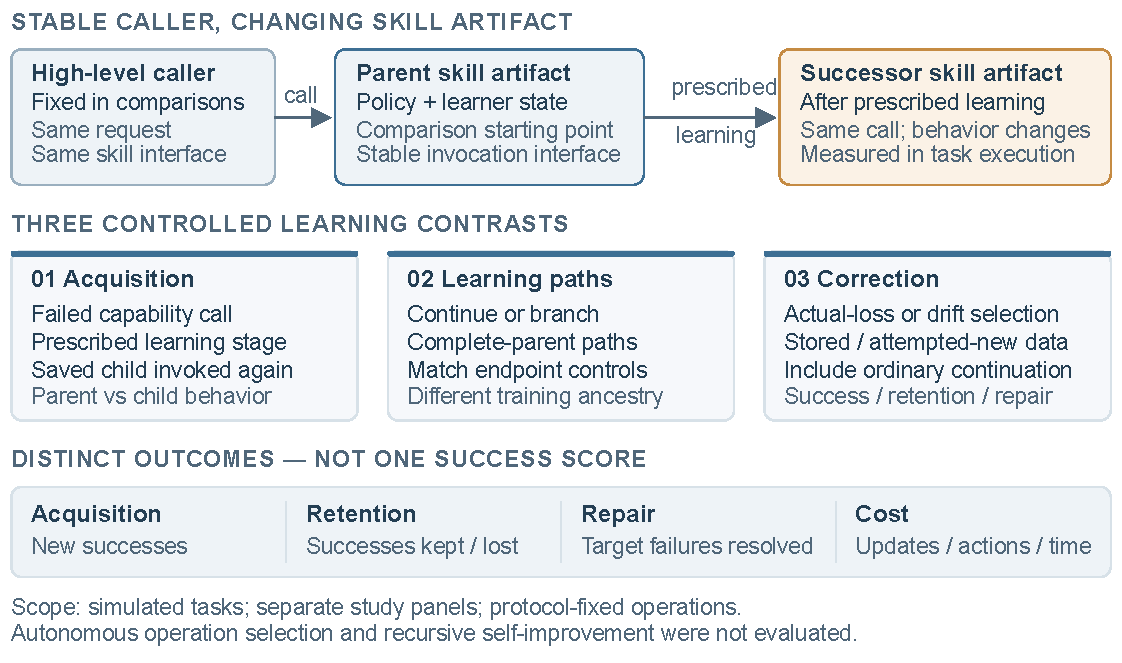
\includegraphics[width=\linewidth]{figures/Fig1.pdf}
\caption{\textbf{Study map.} A fixed high-level caller accesses parent and
successor skill policies through the same interface. Three prescribed
learning contrasts examine acquisition, complete-parent paths and
corrective experience. Outcomes distinguish new success, retention,
target repair and measured cost. The schematic summarizes prescribed
experiments; autonomous operation selection and recursive improvement
were not evaluated. Study panels remain separate.}
\end{figure}
\FloatBarrier

Choosing how to update a skill requires a comparison with the learning
operations already available to the system. Continuing a shared policy,
creating a specialist and collecting corrective demonstrations can
produce different successors even when the next call uses the same skill
name. The relevant outcome includes newly solved cases, lost parent
successes and whether the motivating failure was repaired. We compare
these outcomes while tracking the complete parent and the supervision
used to produce each child.

Execution-driven robot improvement and continual learning already
address related problems. Agentic systems use failures or successful
executions to obtain new policies and reusable skills; replay and
structural expansion address adaptation and forgetting
\cite{wang2026searselfevolvingagenticrobotics, xiao2026enpireagenticrobotpolicy, wen2026roborsistableefficientreusable, pmlr-v97-li19m, pmlr-v164-yang22a}.
We do not propose the general idea of execution feedback, replay or
skill growth. Instead, we examine the following empirical question:
\textbf{how do complete-parent choices and feedback-selected experience
change acquired and retained behavior under a fixed capability
interface, once simple learning alternatives are included?}

Three controlled contrasts organize the answer. First, a native
acquisition study connects a failed capability call to a prescribed
learning stage and subsequent invocation of the saved child. Second, a
multi-cycle study compares learning paths with matched endpoint
architecture, endpoint count and path-level update allocations. Its
branch comparison also fixes the first-request task's final checkpoint,
exposing the remaining second-task difference without attributing it to
an individual optimizer or state component. Third, a correction study
fixes the complete starting policy and learner, then crosses experience
selection with supervision acquisition while retaining ordinary
continuation as a control. The studies have different frozen scene
panels; their case counts are reported separately.

The paper contributes the following bounded evidence:

\begin{itemize}
\tightlist
\item
  A traced capability-acquisition instance with paired new-scene
  evaluation, showing both clear acquisition and concrete prior-success
  losses behind stable calls.
\item
  A matched-endpoint comparison that measures the size, direction and
  reversals of complete-parent learning-path differences across two
  request streams and six continuation roots.
\item
  A fixed correction experiment that separates total success, retention
  and target repair while testing actual-loss versus action-mean drift
  selection and stored versus attempted-new supervision against ordinary
  continuation.
\end{itemize}

The contrasts separate evidence of capability change from evidence for
choosing a learning operation. The Can gain establishes the former in
one lineage. Selecting a parent or collecting targeted experience
requires the corresponding controlled comparison. The branch reversals
and correction results do not establish a generally preferable
operation. They show why a system designer needs the measured parent
losses and target outcomes alongside total success, with ordinary
continuation retained when assessing the added value of corrective
experience.

All experiments use known simulated tasks, explicit task identifiers and
protocol-fixed learning rules. The evaluated object is the learned skill
artifact; autonomous operation selection and physical deployment are
outside the measured scope.

\section{Related work}\label{related-work}

\subsection{Execution-driven capability
improvement}\label{execution-driven-capability-improvement}

SEAR, ENPIRE and RoboRSI provide direct precedents for using execution
experience in robot-policy or skill improvement
\cite{wang2026searselfevolvingagenticrobotics, xiao2026enpireagenticrobotpolicy, wen2026roborsistableefficientreusable}.
F4R connects deployment failures, reconstructed training conditions,
corrective demonstrations, policy refinement and redeployment. Its
cross-task evaluation includes degradation after a targeted update
followed by repair through another feedback-driven cycle
\cite{yu2026f4r}. These works rule out treating failure feedback or
learned-policy exposure to an agent as new by themselves. Our recurrent
behavior-cloning experiments do not reproduce their complete learning
pipelines or compare methods by importing their reported success rates.

Autonomous robot improvement also has earlier learning-system
precedents. MEDAL++ learns forward and backward policies together with
reward classifiers from demonstrations and autonomous interaction, while
retaining initial and intermittent manual resets in its real-robot
procedure \cite{pmlr-v229-sharma23b}. SOAR keeps its high-level
vision-language and image-subgoal models frozen, selects feasible tasks
from a given task list to guide collection, and improves a low-level
goal-conditioned policy with success-filtered, hindsight-relabelled data
mixed with pretraining data \cite{pmlr-v270-zhou25b}. A fixed
high-level model with a learning skill layer is therefore not a new
structure by itself. Our experiments compare prescribed complete-parent
and corrective-data choices and report prior-success losses and costs;
they do not reproduce either autonomous acquisition pipeline or treat
old-data mixing as proof of retention.

AdaRSI first refines the harness, then uses counterfactual re-execution
to identify sub-steps for weight adaptation \cite{wang2026adarsi}. Its
controls include training every sub-step, prioritizing the
lowest-success sub-steps and substituting the base policy into the final
procedure. Paired tests also report that fine-tuning can degrade motions
the base policy already performs. These results address procedure
effects, policy changes and losses on previously successful motions. Our
fixed-caller comparisons instead intervene on complete-parent learning
paths and corrective-data choices; they do not reproduce AdaRSI or
establish superiority over it.

EmbodiRSI uses rollout feedback for corrective experience and targeted
recollection, with a static-collection comparison at matched
retained-trajectory counts \cite{lang2026embodirsi}. Its rounds and
retained-data quotas are fixed in advance; feedback changes experience
acquisition within that schedule. Thus an experience-driven loop need
not select its own optimizer or number of rounds. Our correction study
compares fixed experience sets and learned outcomes rather than
implementing EmbodiRSI's recovery and collection pipeline. Matched
retained counts in that prior study should not be read as matching every
collection attempt or computational cost.

Persistent experience can change robot execution while model weights
remain fixed. ReTrace retains validated corrections and failure lessons
through an executor--attributor loop \cite{yu2026retrace}. AGP reuses
saved programs and task knowledge in fresh execution contexts; its
repeated-trial analysis notes that an empty-experience control is needed
to isolate reuse from ordered scene changes
\cite{jia2026agentaspolicy}. FastHarness instead keeps the VLA policy
frozen and changes its supervision schedule using stage memory and
reviewed outcomes \cite{lin2026fastharness}. These precedents
distinguish retained skill knowledge and adaptive supervision from
policy training. Our experiments prescribe recurrent-policy updates and
examine their behavioral consequences; they do not establish autonomous
update selection or a general efficiency advantage over these systems.

Execution experience can also improve code artifacts. EmbodiedEvo
retains code Skills and diagnostic Lessons while keeping the model
weights and robot interface fixed
\cite{li2026embodiedevoselfimprovingcodingagents}. COAP develops a
stateful robot-code library through coding-agent revisions
\cite{hu2026embodied}. Our experiments intervene on complete
policy-training states and their learning data. That difference defines
the studied artifact; it does not establish that policy-based
improvement is a new alternative to code-based improvement.

EmbodiedRSI maintains competing code and skill hypotheses and chooses
experiments to distinguish them \cite{song2026embodiedrsi}. Its matched
trials connect outcomes to candidate changes. Our experiments fix the
learning operations and examine their behavioral consequences; they do
not implement hypothesis-guided autonomous experiment selection.

ASPIRE uses a coordinator--actor workflow to refine robot programs from
execution traces and consolidate validated repair patterns in a reusable
skill library \cite{lu2026aspire}. SHAPER uses a frozen model in
planner and optimizer roles to evolve textual skills and a context
harness while leaving planner and executor weights unchanged
\cite{wang2026shaper}. These systems provide precedents for role
separation and execution-driven skill improvement. Our experiments
update recurrent policy-training states under prescribed operations and
do not evaluate either program-search system.

RoboFoundry treats context and hierarchical skills as parts of an
evolving agent system and converts execution traces into persistent
system changes
\cite{liang2026robofoundrysystemaspolicyevolutionselflearning}.
Skill-space shooting searches for corrective trials through reusable
skills and turns successful trials into policy supervision
\cite{rui2026skillspaceshootingautonomousrobot}. These works connect
skill reuse to improvement from execution. Our contrasts prescribe the
operations and feedback sets; they do not evaluate autonomous correction
search or system-wide evolution.

\subsection{Learning paths and continual skill
adaptation}\label{learning-paths-and-continual-skill-adaptation}

Learn to Grow selects among reuse, adaptation and additional structure
\cite{pmlr-v97-li19m}. LOTUS combines continual skill discovery,
hierarchical imitation learning and replay; CLARE and IsCiL study
adapter retrieval, routing or expansion for continued task adaptation
\cite{wan2024lotuscontinualimitationlearning, roemer2026clare, lee2024iscil}.
Yang and colleagues compare lifelong-learning methods on robotic tasks
under approximately matched training interaction and different task
orders \cite{pmlr-v164-yang22a}. Freezing, expanding, replaying and
measuring forgetting therefore are established operations. Our matched
branching contrast specifies which endpoint and allocation controls are
held fixed and reports the residual second-task outcomes in this
particular system.

Yu and colleagues combine multimodal latent replay with an
angular-margin feature-adjustment loss; their continual stage updates
the temporal decoder and policy head while keeping the earlier
representation modules frozen
\cite{yu2026lifelongimitationlearningmultimodal}. In their 2025 OMLA
preprint, Zhu and colleagues freeze the pretrained policy and learn
task-specific adapters through an old-task meta-learning stage followed
by new-task fine-tuning
\cite{zhu2025efficientcontinualadaptationpretrained}. These methods
distinguish retaining prior behavior from using prior tasks to improve
subsequent adaptation. Our recurrent BC comparisons do not evaluate
either representation regularization or meta-learned adapter
initialization.

Liu and colleagues find that large-scale pretraining changes continual
robot learning and that simple replay can preserve earlier performance
in pretrained VLAs \cite{liu2026pretrainedcontinual}. Their comparisons
include smaller behavior-cloning policies and initialization controls
within a VLA architecture. Our task-pretrained recurrent BC model
differs from their scratch-trained policies and broadly pretrained VLAs.
The present branching and correction results do not establish the same
trade-offs for foundation policies.

Complete learning state also has precedent as an experimental object.
Guo differentiates short training trajectories through model and
optimizer state and studies interactions with future minibatch schedules
\cite{guo2026delayedoptimizerstatetransportshapes}. Our intervention
changes a complete parent, bundling model, optimizer and sampling
history. It does not isolate that work's optimizer-specific mechanism or
claim training-history dependence as a newly discovered principle.

Recent robot studies also make simple replay and inherited learners
substantive controls. Zhu and colleagues study experience replay across
ten physical manipulation tasks, including heterogeneous task streams
and replay schedules \cite{zhu2026continualvla}. ACCRUE carries
actor--critic networks across tasks and preserves earlier behavior
through cached actor targets \cite{kim2026accrue}. These precedents
already address sustained learning and retention. Here the
complete-parent comparison concerns bundled behavior-cloning states, and
the correction comparison asks whether selected corrective experience
adds benefit over BC continuation with existing target replay; neither
comparison establishes a new general inheritance or replay principle.

\subsection{Interference signals and corrective
supervision}\label{interference-signals-and-corrective-supervision}

CLASP constructs demonstration-anchored regions from demonstration and rollout states, combines local imitation difficulty with coverage to guide novice demonstrations, and reweights training through the same region map \cite{pmlr-v306-zhu26s}. Our correction study instead compares fixed supervision sets selected by observed success losses or same-input action-mean drift, alongside ordinary continuation. These differences define the evaluated interventions; they do not establish an advantage over CLASP or make the limited learning utility of task-valid demonstrations a new principle.

MIR selects memories most affected by an anticipated update and includes
a generative variant \cite{aljundi2019mir}. RIFAR compares action
predictions before and after adaptation on identical historical inputs,
then reselects reliable generated replay; its latest version explicitly
distinguishes action drift from forgetting \cite{lin2026rifar}. RECALL
collects recovery demonstrations from uncertain states and examines
replay and regularization for preserving earlier tasks
\cite{karli2026recall}. We use a low-dimensional action-mean drift
adaptation as a comparison signal, not a reproduction of full RIFAR. The
correction experiment tests the utility of the resulting experience
choices and an attempted-new-with-fallback acquisition strategy against
stored successful executions and ordinary continuation.

Memory Anchors identifies old experiences where observations have
overlapping representations but the tasks require conflicting actions,
then tests their role in retaining earlier robot behaviors
\cite{du2026memoryanchorscontinualrobot}. Our observed-loss and
action-mean-drift selections measure different signals. They do not
reproduce that representation-based rule or establish superiority over
it.

Historical-policy rehearsal also has established precedent. CLEAR adds
historical-policy cloning within an actor--critic replay method
\cite{NEURIPS2019_fa7cdfad}. The D diagnostic used to initialize our
correction study adapts the policy-distribution preservation rationale
to imitation learning, without reproducing CLEAR's value cloning or
V-Trace learning. Its construction and failures are reported in Appendix
A.

\subsection{Boundary with runtime
governance}\label{boundary-with-runtime-governance}

Earlier AEROS work studies lifecycle-time compatibility, activation and
rollback, while related regression-test-selection work examines the
replacement of already-trained module versions
\cite{qin2026governedcapabilityevolution, qin2026regressiontestselectionupdated}.
The interventions here precede that replacement decision: they determine
which capability artifact learning produces. Version binding and
execution records support the experiment, but governance, contracts and
regression-test selection are not claimed as new contributions of this
paper.

\section{Materials and methods}\label{materials-and-methods}

\subsection{Calls, execution and
learning}\label{calls-execution-and-learning}

Let \(C\) be the set of named capability calls and let \(\rho\) map a
call to its current artifact. An artifact identifies its policy
checkpoint, declared task scope and provenance. A complete learning
state \(S\) includes model weights, optimizer and scheduler state,
random-number streams, samplers, counters, model modes and the recurrent
fields in the frozen checkpoint schema. A file name alone does not
establish this identity.

The high-level caller requests a skill and receives its result. The
executor maintains the active policy and recurrent state during the
call, subject to completion, failure, timeout and guard conditions.
Learning operates outside that invocation and produces a candidate child
for later calls. This is a division of responsibilities, not evidence
that the current experimental coordinator is an autonomous learning
agent. In the acquisition study, AEROS invokes the saved artifact; later
controlled studies evaluate frozen checkpoints through the native
backend.

An invocation record binds the requested capability, the artifact
actually used, the episode outcome and resource counters. A learning
request identifies the admitted parent and the execution evidence that
motivated the operation. The learner restores that parent, applies the
specified operation and saves the child. The experiment then measures
the child rather than inferring capability from training loss or from a
successful interface call.

For a shared update \(A\rightarrow A'\), only calls currently routed to
\(A\) change their route. For a specialist branch on capability \(c\),
the complete admitted parent is copied, the branch is trained, and only
\(\rho(c)\) changes. Declared task scope and current route ownership are
different: a formerly shared state can remain installed for one task
after another task has acquired a branch. The current implementation
uses a single coordinator with isolated workers and provenance checks;
no distributed transaction or production crash-safety claim is made.

\subsection{What each contrast
controls}\label{what-each-contrast-controls}

Table 1 summarizes the intervention and fixed controls for each study.

\begin{longtable}[]{@{}
  >{\raggedright\arraybackslash}p{(\linewidth - 6\tabcolsep) * \real{0.2500}}
  >{\raggedright\arraybackslash}p{(\linewidth - 6\tabcolsep) * \real{0.2500}}
  >{\raggedright\arraybackslash}p{(\linewidth - 6\tabcolsep) * \real{0.2500}}
  >{\raggedright\arraybackslash}p{(\linewidth - 6\tabcolsep) * \real{0.2500}}@{}}
\caption{Overview of the three controlled learning contrasts. The
experiments address different stages and do not share one pooled
evaluation panel.}\tabularnewline
\toprule\noalign{}
\begin{minipage}[b]{\linewidth}\raggedright
Study
\end{minipage} & \begin{minipage}[b]{\linewidth}\raggedright
Intervention
\end{minipage} & \begin{minipage}[b]{\linewidth}\raggedright
Fixed controls
\end{minipage} & \begin{minipage}[b]{\linewidth}\raggedright
Main observed outcome
\end{minipage} \\
\midrule\noalign{}
\endfirsthead
\toprule\noalign{}
\begin{minipage}[b]{\linewidth}\raggedright
Study
\end{minipage} & \begin{minipage}[b]{\linewidth}\raggedright
Intervention
\end{minipage} & \begin{minipage}[b]{\linewidth}\raggedright
Fixed controls
\end{minipage} & \begin{minipage}[b]{\linewidth}\raggedright
Main observed outcome
\end{minipage} \\
\midrule\noalign{}
\endhead
\bottomrule\noalign{}
\endlastfoot
Acquisition & Prescribed replay stage after failed Can calls & Frozen
parent/child endpoints and paired recorded initial conditions & New
successes and lost prior successes \\
Complete-parent paths & Early versus delayed branch formation & Final
architecture/count, path updates, task-window allocation and first-task
final endpoint & Residual second-task outcomes and reversals \\
Corrective experience & Actual-loss/drift selection crossed with
stored/attempted-new targets & Complete D parent, BC learner, update
budget and common original/target windows & Total success, retained
parent cases and target repair \\
\end{longtable}

The learner and demonstration data use the robomimic framework
\cite{pmlr-v164-mandlekar22a}. Task identifiers are explicit;
observation semantics are not inferred by a language model. The
shared-interface experiments use fixed native success, action horizons
and guards. The correction study uses a 23-dimensional low-dimensional
observation vector and seven control outputs; exact field order, model
configuration, split identities and state bindings are preserved in its
protocol. Equal dimensions do not establish transfer between tasks.

\subsection{Outcome definitions and
interpretation}\label{outcome-definitions-and-interpretation}

For each paired panel, an acquisition is a parent failure followed by a
child success; a loss is a parent success followed by a child failure.
Retention uses the successful parent cases as its denominator. A higher
total success count can therefore coexist with lost previous successes.
Target repair refers to the particular development scene motivating a
correction and is reported separately from a larger panel.

Recorded initial-state checks include flattened simulator-state digests,
model XML and control settings as specified by each protocol. They do
not prove equality of every internal MuJoCo field. All success criteria
and guards are retained across compared endpoints. The studies report
independent units according to their design: scene pairs for
fixed-endpoint observations, continuation roots for the prespecified
multi-cycle tests, and a single learning lineage for the correction
experiment. Scene counts and reused training nodes do not create
additional independent training replications.

The comparisons test particular learning interventions. Capacity
matching does not isolate an individual state component, and matching
update counts does not equalize all data exposure or total cost. The
acquisition study establishes that learning occurred; the later
contrasts address which aspects can be attributed to a specified path or
corrective-data choice.

\subsection{AI-assisted preparation}\label{ai-assisted-preparation}

AI tools (OpenAI Codex and OpenClaw) assisted with software development and manuscript revision. Outputs were checked against primary sources, execution records and source code; the authors are responsible for the work.

\section{Experiments and results}\label{experiments-and-results}

The experiments comprise capability acquisition (Study 1),
complete-parent learning paths (Study 2), and corrective experience
(Study 3). Each study has its own fixed protocol and evaluation panel;
results are reported separately. We describe the task settings,
comparison variants, outcomes and resources below.

\subsection{Capability acquisition through
AEROS}\label{capability-acquisition-through-aeros}

The native experiments use the robomimic learning framework and
demonstration data described by Mandlekar and colleagues
\cite{pmlr-v164-mandlekar22a}. The recurrent behavior-cloning
configuration and native runtime are fixed by the experiment artifacts;
the citation attributes the framework and data rather than verifying a
particular installed version.

The initial policy served Can and Square. On four development scenes per
task, it solved no Can scene and two Square scenes. The Can failure
initiated one predefined replay stage of 20,000 updates with equal Can
and Square training windows. The learner used existing demonstrations;
execution feedback only determined whether to start this operation. The
saved child was then invoked through AEROS and solved four Can scenes
and one Square scene.

Direct invocation of the same child matched the eight agent-invoked
episodes on outcomes, step counts, success holds, stop reasons and
recorded initial state/model identities. Complete action trajectories
were not compared. This checks the deployed learning connection; it is
not a superiority comparison against another learning method.

After sealing the two endpoints, the protocol evaluated 32 new initial
scenes per task. Parent and child shared matching recorded flattened
simulator states, model XML and control limits for each pair. Within
each task, the 32 initial-state digests were distinct. These checks do
not cover every internal MuJoCo data field. Success required five
consecutive native-success checks within the fixed 400-action horizon
and guards.

Table 2 reports the paired outcomes for this single training
realization.

\begin{longtable}[]{@{}
  >{\raggedright\arraybackslash}p{(\linewidth - 10\tabcolsep) * \real{0.1304}}
  >{\raggedleft\arraybackslash}p{(\linewidth - 10\tabcolsep) * \real{0.1739}}
  >{\raggedleft\arraybackslash}p{(\linewidth - 10\tabcolsep) * \real{0.1739}}
  >{\raggedleft\arraybackslash}p{(\linewidth - 10\tabcolsep) * \real{0.1739}}
  >{\raggedleft\arraybackslash}p{(\linewidth - 10\tabcolsep) * \real{0.1739}}
  >{\raggedleft\arraybackslash}p{(\linewidth - 10\tabcolsep) * \real{0.1739}}@{}}
\caption{Paired endpoint results on 32 new initial scenes per task.
Gains and losses compare the child with its parent. Paired p values use
two-sided exact binomial tests on discordant parent--child outcomes,
with Holm adjustment across the two tasks.}\tabularnewline
\toprule\noalign{}
\begin{minipage}[b]{\linewidth}\raggedright
Task
\end{minipage} & \begin{minipage}[b]{\linewidth}\raggedleft
Parent
\end{minipage} & \begin{minipage}[b]{\linewidth}\raggedleft
Child
\end{minipage} & \begin{minipage}[b]{\linewidth}\raggedleft
Paired gains
\end{minipage} & \begin{minipage}[b]{\linewidth}\raggedleft
Paired losses
\end{minipage} & \begin{minipage}[b]{\linewidth}\raggedleft
Holm-adjusted paired p
\end{minipage} \\
\midrule\noalign{}
\endfirsthead
\toprule\noalign{}
\begin{minipage}[b]{\linewidth}\raggedright
Task
\end{minipage} & \begin{minipage}[b]{\linewidth}\raggedleft
Parent
\end{minipage} & \begin{minipage}[b]{\linewidth}\raggedleft
Child
\end{minipage} & \begin{minipage}[b]{\linewidth}\raggedleft
Paired gains
\end{minipage} & \begin{minipage}[b]{\linewidth}\raggedleft
Paired losses
\end{minipage} & \begin{minipage}[b]{\linewidth}\raggedleft
Holm-adjusted paired p
\end{minipage} \\
\midrule\noalign{}
\endhead
\bottomrule\noalign{}
\endlastfoot
Can & 0/32 & 30/32 & 30 & 0 & \(3.7253\times 10^{-9}\) \\
Square & 16/32 & 19/32 & 7 & 4 & 0.548828125 \\
\end{longtable}

Can acquisition extended beyond the four development scenes. The child's
success rate was 93.75\%, with a Wilson 95\% interval of approximately
79.85--98.27\%; two failures remain. Square's total increased, but four
previously successful scenes were lost. Its paired test neither
established a change nor demonstrated equivalence or absence of
forgetting. Both tasks participated in replay, so new Square successes
cannot be attributed specifically to learning Can.

The acquisition stage used 20,000 optimizer updates, two million
training windows and 5,912 policy actions in 258.344 seconds. The
separate endpoint evaluation added no training and used 30,801 actions
in 483.363 seconds. Neither stage used a model-service call. Checkpoint
identities, invocation events and case summaries were checked for
consistency; these checks did not independently repeat neural inference
or evaluate the success predicate in another simulator.

\subsection{Complete-parent learning
paths}\label{complete-parent-learning-paths}

\subsubsection{Fixed design and independent
units}\label{fixed-design-and-independent-units}

The main comparison measures the size and direction of final
task-outcome differences between complete-state branching schedules with
matched endpoint capacity and path-level update allocations. Shared
fine-tuning and replay provide context for acquisition and preservation
over repeated calls. Six continuation random roots (101, 211, 307, 401,
503 and 601) share one pretrained Square weight source. They are
distinct continuation random states, not six independently pretrained
models. Each root has two request streams, Can→Square→Can and
Square→Can→Square, with three 5,000-update events per stream.

Shared fine-tuning uses 100 windows from the requested task per update.
Shared experience replay (ER; labelled replay in the tables) uses 50 Can
and 50 Square windows. Early branching copies the complete parent at the
first request when it still serves both tasks; delayed branching first
updates the shared parent and branches at a later request if it remains
shared. A complete copy includes optimizer and random streams, rather
than only weights. The rules are prescribed by the experimenter.
Existing demonstrations supply supervision; execution feedback does not
choose the update rule or its quota. All three learning events occur
according to the fixed schedule, including events whose preceding
requested-task evaluation has already succeeded. This comparison
therefore differs from the single failure-triggered instance in Section
4.1.

The learner is a two-layer 400-unit LSTM behavior-cloning policy with a
five-component Gaussian-mixture head, trained with Adam at learning rate
0.0001. It uses low-dimensional robot/object observations and an
explicit two-element task identifier. Can training comprises 180
demonstrations and Square training 160; each update samples ten-step
windows. All demonstration samples receive unit loss weight. With the
auxiliary mixture term disabled, the objective is the mean negative log
likelihood of the demonstrated actions. Camera perception and semantic
task inference are outside this experiment. The accompanying protocol
records full observation shapes, exact split identities, state
provenance, native execution conditions and reproduction limitations.

The implementation contains 48 logical paths and 144 learning events
with 66 unique physical training nodes. A node can be reused only when
its complete parent and fixed learning inputs match. This reuse does not
create independent training replications. Each logical path has 15,000
updates, but the actual experiment uses 330,000 updates, rather than the
720,000 updates obtained by summing duplicated logical paths.

Final evaluation uses 32 paired initial scenes per task. These scenes
exclude the earlier development and single-instance endpoint panels. A
common baseline is evaluated before training, but its observations are
not consumed by the fixed learning rules. All learned states and
terminal routes are sealed before final endpoint evaluations. The
baseline succeeds in 0/32 Can and 19/32 Square scenes; these are
different panels from Table 2. No endpoint, recipe or random seed is
selected from final results.

The six continuation roots are the inferential units. Within a root, two
tasks and two streams contribute equally to an aggregate final success
count out of 128. The same scene panels, request streams and reused
nodes are dependent observations, not additional independent roots. The
prespecified comparisons are replay minus fine-tuning and early minus
delayed branching, using two-sided exact sign tests after removing ties
and Holm correction across the two tests.

\subsubsection{Acquisition and prior-success
loss}\label{acquisition-and-prior-success-loss}

Table 3 gives descriptive task-level totals. Each task denominator of
384 repeats the same 32-scene panel across six roots and two streams; it
is not an independent sample size of 384. Square has 228 initially
successful case occurrences under this repeated-panel accounting. Can
retention is undefined because its initial success denominator is zero.

\begin{longtable}[]{@{}
  >{\raggedright\arraybackslash}p{(\linewidth - 10\tabcolsep) * \real{0.20}}
  >{\raggedleft\arraybackslash}p{(\linewidth - 10\tabcolsep) * \real{0.16}}
  >{\raggedleft\arraybackslash}p{(\linewidth - 10\tabcolsep) * \real{0.16}}
  >{\raggedleft\arraybackslash}p{(\linewidth - 10\tabcolsep) * \real{0.16}}
  >{\raggedleft\arraybackslash}p{(\linewidth - 10\tabcolsep) * \real{0.16}}
  >{\raggedleft\arraybackslash}p{(\linewidth - 10\tabcolsep) * \real{0.16}}@{}}
\caption{Descriptive repeated-panel totals for the completed multi-cycle
comparison. Gains and losses compare each final result with the
corresponding common-baseline case.}\tabularnewline
\toprule\noalign{}
\begin{minipage}[b]{\linewidth}\raggedright
Fixed rule
\end{minipage} & \begin{minipage}[b]{\linewidth}\raggedleft
Can final /384
\end{minipage} & \begin{minipage}[b]{\linewidth}\raggedleft
Square final /384
\end{minipage} & \begin{minipage}[b]{\linewidth}\raggedleft
Square gains
\end{minipage} & \begin{minipage}[b]{\linewidth}\raggedleft
Square losses /228
\end{minipage} & \begin{minipage}[b]{\linewidth}\raggedleft
Square old-success retention
\end{minipage} \\
\midrule\noalign{}
\endfirsthead
\toprule\noalign{}
\begin{minipage}[b]{\linewidth}\raggedright
Fixed rule
\end{minipage} & \begin{minipage}[b]{\linewidth}\raggedleft
Can final /384
\end{minipage} & \begin{minipage}[b]{\linewidth}\raggedleft
Square final /384
\end{minipage} & \begin{minipage}[b]{\linewidth}\raggedleft
Square gains
\end{minipage} & \begin{minipage}[b]{\linewidth}\raggedleft
Square losses /228
\end{minipage} & \begin{minipage}[b]{\linewidth}\raggedleft
Square old-success retention
\end{minipage} \\
\midrule\noalign{}
\endhead
\bottomrule\noalign{}
\endlastfoot
Shared fine-tuning & 179 & 105 & 29 & 152 & 33.33\% \\
Shared replay & 310 & 260 & 70 & 38 & 83.33\% \\
Early branching & 356 & 277 & 72 & 23 & 89.91\% \\
Delayed branching & 350 & 261 & 75 & 42 & 81.58\% \\
\end{longtable}

Replay and branching improve aggregate outcomes relative to shared
fine-tuning in this setting, but every rule loses initially successful
Square cases. Early branching has the largest descriptive final success
total, while delayed branching has more newly gained Square cases.
Neither observation establishes universal dominance or preservation of
every earlier capability.

Table 4 shows all root-level outcomes and the two prespecified
contrasts. The mean rate differences are 0.3723958333 for replay minus
fine-tuning and 0.0286458333 for early minus delayed branching.

\begin{longtable}[]{@{}
  >{\raggedright\arraybackslash}p{(\linewidth - 12\tabcolsep) * \real{0.18}}
  >{\raggedleft\arraybackslash}p{(\linewidth - 12\tabcolsep) * \real{0.15}}
  >{\raggedleft\arraybackslash}p{(\linewidth - 12\tabcolsep) * \real{0.12}}
  >{\raggedleft\arraybackslash}p{(\linewidth - 12\tabcolsep) * \real{0.12}}
  >{\raggedleft\arraybackslash}p{(\linewidth - 12\tabcolsep) * \real{0.13}}
  >{\raggedleft\arraybackslash}p{(\linewidth - 12\tabcolsep) * \real{0.13}}
  >{\raggedleft\arraybackslash}p{(\linewidth - 12\tabcolsep) * \real{0.17}}@{}}
\caption{Final successes aggregated over two tasks and two streams
within each continuation root. The 128 case occurrences form a
root-level outcome, not 128 independent replications.}\tabularnewline
\toprule\noalign{}
\begin{minipage}[b]{\linewidth}\raggedright
Continua\-tion root
\end{minipage} & \begin{minipage}[b]{\linewidth}\raggedleft
Fine-tuning /128
\end{minipage} & \begin{minipage}[b]{\linewidth}\raggedleft
Replay /128
\end{minipage} & \begin{minipage}[b]{\linewidth}\raggedleft
Early /128
\end{minipage} & \begin{minipage}[b]{\linewidth}\raggedleft
Delayed /128
\end{minipage} & \begin{minipage}[b]{\linewidth}\raggedleft
Replay −FT
\end{minipage} & \begin{minipage}[b]{\linewidth}\raggedleft
Early −delayed
\end{minipage} \\
\midrule\noalign{}
\endfirsthead
\toprule\noalign{}
\begin{minipage}[b]{\linewidth}\raggedright
Continua\-tion root
\end{minipage} & \begin{minipage}[b]{\linewidth}\raggedleft
Fine-tuning /128
\end{minipage} & \begin{minipage}[b]{\linewidth}\raggedleft
Replay /128
\end{minipage} & \begin{minipage}[b]{\linewidth}\raggedleft
Early /128
\end{minipage} & \begin{minipage}[b]{\linewidth}\raggedleft
Delayed /128
\end{minipage} & \begin{minipage}[b]{\linewidth}\raggedleft
Replay −FT
\end{minipage} & \begin{minipage}[b]{\linewidth}\raggedleft
Early −delayed
\end{minipage} \\
\midrule\noalign{}
\endhead
\bottomrule\noalign{}
\endlastfoot
101 & 49 & 96 & 112 & 102 & 47 & 10 \\
211 & 51 & 90 & 107 & 102 & 39 & 5 \\
307 & 54 & 100 & 102 & 98 & 46 & 4 \\
401 & 35 & 92 & 106 & 105 & 57 & 1 \\
503 & 50 & 102 & 99 & 97 & 52 & 2 \\
601 & 45 & 90 & 107 & 107 & 45 & 0 \\
\end{longtable}

Replay minus fine-tuning has six positive differences and an unadjusted
two-sided sign-test p of 0.03125. Early minus delayed branching has five
positive differences and one tie, giving p=0.0625. Both Holm-adjusted p
values are 0.0625. Neither comparison reaches 0.05 under the
prespecified tests. The resolution limit was documented before the run;
we do not change test direction, replace the analysis or add roots after
observing results. Nonsignificance does not establish equivalence.

Fig 2 displays the six root-level contrasts on a common percentage-point
scale. Each point is one continuation root; the figure does not add
case-level confidence intervals or a different test.

\begin{figure}[!htbp]
\centering
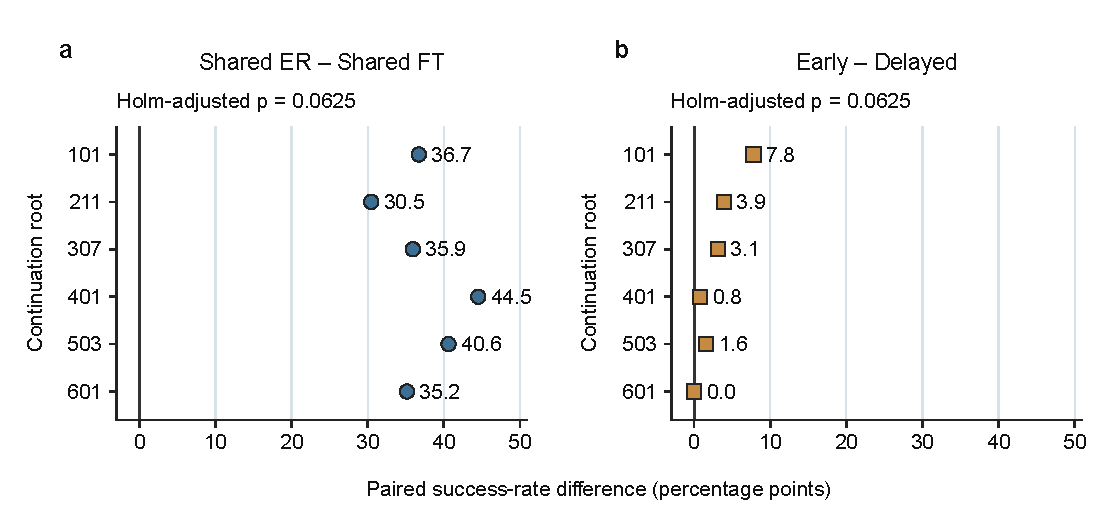
\includegraphics[width=\linewidth]{figures/Fig2.pdf}
\caption{\textbf{Root-level paired differences in final success.} Each panel
shows all six continuation roots after equal aggregation across two
tasks and two streams. The zero line is a reference; both prespecified
Holm-adjusted two-sided sign-test p values are
0.0625.}
\end{figure}
\FloatBarrier

Fig 3 separates newly gained Square successes from initially successful
case occurrences that are lost. These repeated-panel totals are
descriptive; they do not supply independent sample sizes for inference.

\begin{figure}[!htbp]
\centering
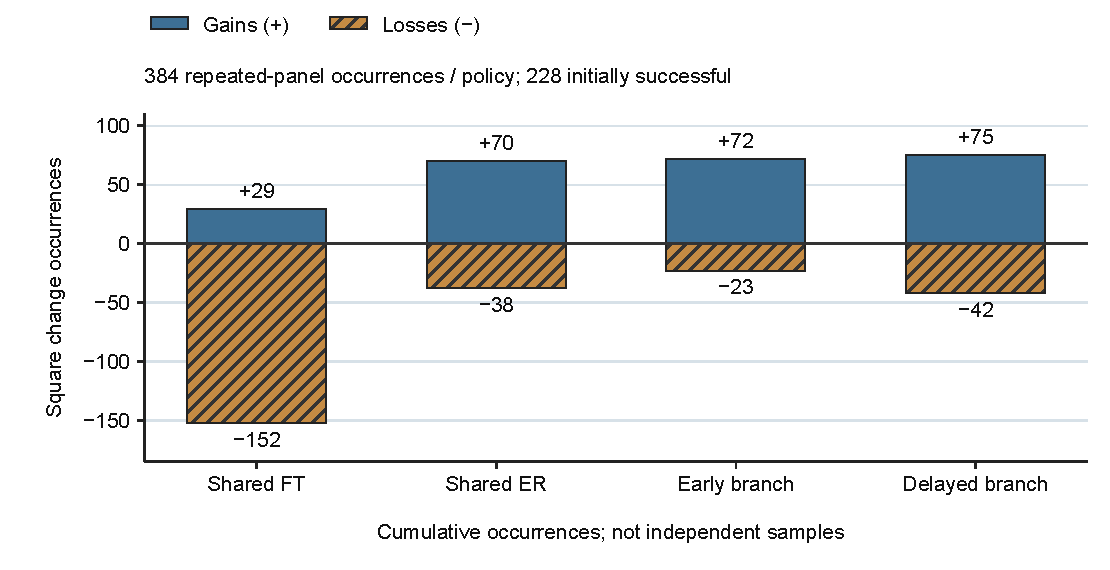
\includegraphics[width=\linewidth]{figures/Fig3.pdf}
\caption{\textbf{Square gains and losses relative to the common baseline.} Each
strategy has 384 repeated-panel case occurrences, including 228
initially successful occurrences. Positive bars count new successes and
negative bars count losses. The counts repeat scene panels across roots
and streams and are not independent training
samples.}
\end{figure}
\FloatBarrier

\subsubsection{Matched-endpoint control and complete-parent
history}\label{matched-endpoint-control-and-complete-parent-history}

Early and delayed branching are matched within all twelve root--stream
pairs on final endpoint count (two), configured architecture and
recorded registered parameter elements (1,996,475 per checkpoint). Both
use 15,000 logical updates and the same allocation of task windows: one
million for the first-request task and 500,000 for the second. These are
allocations across each logical path, not equal task exposure along the
ancestry of each endpoint: the delayed second-task branch additionally
inherits the first shared update. These controls concern the two
branching rules. They do not imply equal exposure or capacity across all
four rules, equal resident memory, or equal total wall time.

The final checkpoint for the first-request task is byte-identical under
early and delayed branching in every pair. The 32 corresponding cases
also agree on all eight prespecified recorded fields. This agreement is
a construction control. The second-request task starts from different
complete parent checkpoints, carrying the consequences of the earlier
shared update under delayed branching. Its comparison therefore holds
final endpoint count and architecture fixed while varying the
complete-parent path. All 48 original recorded-behavior construction
checks pass; neither those checks nor checkpoint digests establish full
action-trajectory equality or a new learning mechanism.

Table 5 reports the final second-task outcomes for both streams and
every root. It is a descriptive decomposition of the prespecified final
endpoint outcomes in Table 4, not a new test or twelve independent
training replications. In Can→Square→Can, the displayed task is Square;
in Square→Can→Square, it is Can.

\begin{longtable}[]{@{}
  >{\raggedright\arraybackslash}p{(\linewidth - 12\tabcolsep) * \real{0.1111}}
  >{\raggedleft\arraybackslash}p{(\linewidth - 12\tabcolsep) * \real{0.1481}}
  >{\raggedleft\arraybackslash}p{(\linewidth - 12\tabcolsep) * \real{0.1481}}
  >{\raggedleft\arraybackslash}p{(\linewidth - 12\tabcolsep) * \real{0.1481}}
  >{\raggedleft\arraybackslash}p{(\linewidth - 12\tabcolsep) * \real{0.1481}}
  >{\raggedleft\arraybackslash}p{(\linewidth - 12\tabcolsep) * \real{0.1481}}
  >{\raggedleft\arraybackslash}p{(\linewidth - 12\tabcolsep) * \real{0.1481}}@{}}
\caption{Second-request-task final successes under the two branching
schedules. Square columns refer to Can→Square→Can and Can columns to
Square→Can→Square. Differences are early minus delayed; all cases use
the original paired panels. The inferential unit remains the
continuation root, with two streams combined as in Table
4.}\tabularnewline
\toprule\noalign{}
\begin{minipage}[b]{\linewidth}\raggedright
Root
\end{minipage} & \begin{minipage}[b]{\linewidth}\raggedleft
Square early /32
\end{minipage} & \begin{minipage}[b]{\linewidth}\raggedleft
Square delayed /32
\end{minipage} & \begin{minipage}[b]{\linewidth}\raggedleft
Difference
\end{minipage} & \begin{minipage}[b]{\linewidth}\raggedleft
Can early /32
\end{minipage} & \begin{minipage}[b]{\linewidth}\raggedleft
Can delayed /32
\end{minipage} & \begin{minipage}[b]{\linewidth}\raggedleft
Difference
\end{minipage} \\
\midrule\noalign{}
\endfirsthead
\toprule\noalign{}
\begin{minipage}[b]{\linewidth}\raggedright
Root
\end{minipage} & \begin{minipage}[b]{\linewidth}\raggedleft
Square early /32
\end{minipage} & \begin{minipage}[b]{\linewidth}\raggedleft
Square delayed /32
\end{minipage} & \begin{minipage}[b]{\linewidth}\raggedleft
Difference
\end{minipage} & \begin{minipage}[b]{\linewidth}\raggedleft
Can early /32
\end{minipage} & \begin{minipage}[b]{\linewidth}\raggedleft
Can delayed /32
\end{minipage} & \begin{minipage}[b]{\linewidth}\raggedleft
Difference
\end{minipage} \\
\midrule\noalign{}
\endhead
\bottomrule\noalign{}
\endlastfoot
101 & 27 & 18 & 9 & 31 & 30 & 1 \\
211 & 24 & 21 & 3 & 30 & 28 & 2 \\
307 & 19 & 17 & 2 & 29 & 27 & 2 \\
401 & 26 & 26 & 0 & 29 & 28 & 1 \\
503 & 24 & 21 & 3 & 26 & 27 & −1 \\
601 & 24 & 25 & −1 & 29 & 28 & 1 \\
\end{longtable}

The two streams expose limits hidden by a nonnegative root-level
aggregate. Delayed branching solves one additional Can case for root 503
and one additional Square case for root 601. Root 601's aggregate tie
combines a −1 and a +1 difference; it does not mean both paths agree.
The streams also exchange the identity of the second task, so their
contrast cannot identify a pure request-order effect.

For the first prespecified root, 101, execution records link all 24
logical learning events to complete parent and child states, installed
routes and subsequent development evaluations. All twelve branching
pairs were also linked to their saved checkpoints and evaluation
records. These checks establish recorded-state consistency without
rerunning learning. Root 101 illustrates the protocol order rather than
a selected best case.

The measured second-task differences remain after the later separation
of route ownership and within the same subsequent update allocation.
Thus matching final capacity and update counts alone does not make these
two observed learning paths interchangeable. The complete history is the
intervention: it includes weights, optimizer, random streams and
samplers. We do not assign the difference to any single component, infer
an irreversible deficit or population-level early-branch advantage, or
identify an optimal or autonomous branch-selection rule.

\subsubsection{Resources and execution
completeness}\label{resources-and-execution-completeness}

All 506 jobs and 48 logical paths complete, with no unknown work
recorded. The physical experiment consumes 330,000 optimizer attempts,
entries and returns; 33,000,000 training windows; 330,000,000 supervised
positions; and 1,003,963 actions and policy inferences. It constructs 72
GPU training-state models and 434 CPU evaluation models, with 4,480
environment constructions and resets. The native batch takes 20,919.084
seconds and makes no model-service calls.

Shared rules retain one complete active endpoint checkpoint per path,
with file sizes approximately 24.38 MB. Branching rules retain two,
totaling approximately 48.75 MB. These are serialized complete-state
file bytes, not measured resident memory. Equal update counts do not
imply equal task-data exposure, model capacity or total cost. Logical
path timing reuses measured node costs and is not an independently
measured wall time for each path; the physical batch total is reported
separately.

\subsection{Corrective experience after an
update}\label{corrective-experience-after-an-update}

In this study, the original Square parent is the frozen 100,000-update
checkpoint. A preceding diagnostic resumed this parent for 1,000 updates
with equal old-observation and target-demonstration windows, replacing
old expert actions with samples from the frozen parent distribution. The
resulting D endpoint repaired the target but lost some earlier
successes. That diagnostic is reported in Appendix A; D is the complete
common starting state for the five continuations below. The final panel
here is different from the acquisition and multi-cycle panels.

D's observed target repair and loss of other successes motivated a
further fixed-protocol comparison. Selector L used the three previously
successful scenes that D failed. Selector F used the three highest
action-mean drift scores among the same nine successful parent
trajectories. Parent and D received identical observation histories,
with the original ten-step recurrent reset horizon. The score was the
upper-20\% temporal mean of the root-mean-square difference between
their analytic Gaussian-mixture action means, divided by the fixed
action range. L and F shared one scene. This is an adaptation of a
drift-selection signal, not full RIFAR; mixture means can cancel changes
among modes and need not be actions taken during execution. The choices
and the budget of three scenes were informed by the earlier exposed
panel, rather than prospectively discovered on the final board.

Supervision condition P used stored successful parent executions from
the selected scenes. Condition G attempted one MimicGen~\cite{Mandlekar2023MimicGen} demonstration
per selected initial scene and used the stored parent execution as a
declared fallback on ordinary task failure. Physical acquisition covered
the five-scene union once: four attempts succeeded and one failed,
consuming 787 actions. LG consequently used three generated
demonstrations; FG used two generated demonstrations and one fallback. G
is therefore an acquisition strategy, not uniformly a fresh-data-only
condition.

Each corrective arm resumed the complete D state for 1,000 updates,
using batches of forty original-data windows, forty existing
target-demonstration windows and twenty selected corrective windows. C0
used twenty additional original-data windows in place of correction. The
common actual-action objective differs from D's preceding
teacher-rehearsal objective, so C0 minus D does not isolate extra
training duration. Full-log checks confirmed that the shared forty
original-data and forty target windows matched at every update across
all five arms. Each arm used its final endpoint; all endpoints were
sealed before evaluation. Equal updates and supervised positions do not
imply equal selection, acquisition or total cost.

Parent, D and the five learned endpoints were evaluated on the same
thirty-two fixed new seeds and four original development seeds under the
existing native hold5 criterion. Initial-state digests were distinct
within the board and matched across endpoints. No new-board digest
matched the eighty bound historical digests, but that comparison is not
an exhaustive proof of unseen physical states. The experiment contains
one training lineage and one paired action stream per scene.

Table 6 reports every endpoint, including both learning-parent
references and ordinary continuation.

\begin{longtable}[]{@{}
  >{\raggedright\arraybackslash}p{(\linewidth - 10\tabcolsep) * \real{0.1364}}
  >{\raggedleft\arraybackslash}p{(\linewidth - 10\tabcolsep) * \real{0.1818}}
  >{\raggedleft\arraybackslash}p{(\linewidth - 10\tabcolsep) * \real{0.1818}}
  >{\raggedleft\arraybackslash}p{(\linewidth - 10\tabcolsep) * \real{0.1818}}
  >{\raggedleft\arraybackslash}p{(\linewidth - 10\tabcolsep) * \real{0.1818}}
  >{\raggedright\arraybackslash}p{(\linewidth - 10\tabcolsep) * \real{0.1364}}@{}}
\caption{Fixed correction-selection and acquisition-strategy comparison.
Retention uses the original parent's twenty-two successful cases as its
denominator; gains and losses compare each endpoint with the original
parent on this new board. The original target belongs to the
separate development panel.}\tabularnewline
\toprule\noalign{}
\begin{minipage}[b]{\linewidth}\raggedright
Endpoint
\end{minipage} & \begin{minipage}[b]{\linewidth}\raggedleft
New-board success
\end{minipage} & \begin{minipage}[b]{\linewidth}\raggedleft
Parent successes retained
\end{minipage} & \begin{minipage}[b]{\linewidth}\raggedleft
Gains / losses vs parent
\end{minipage} & \begin{minipage}[b]{\linewidth}\raggedleft
Development success
\end{minipage} & \begin{minipage}[b]{\linewidth}\raggedright
Original target
\end{minipage} \\
\midrule\noalign{}
\endfirsthead
\toprule\noalign{}
\begin{minipage}[b]{\linewidth}\raggedright
Endpoint
\end{minipage} & \begin{minipage}[b]{\linewidth}\raggedleft
New-board success
\end{minipage} & \begin{minipage}[b]{\linewidth}\raggedleft
Parent successes retained
\end{minipage} & \begin{minipage}[b]{\linewidth}\raggedleft
Gains / losses vs parent
\end{minipage} & \begin{minipage}[b]{\linewidth}\raggedleft
Development success
\end{minipage} & \begin{minipage}[b]{\linewidth}\raggedright
Original target
\end{minipage} \\
\midrule\noalign{}
\endhead
\bottomrule\noalign{}
\endlastfoot
Parent & 22/32 & 22/22 & reference & 3/4 & fail \\
D & 21/32 & 17/22 & +4 / -5 & 4/4 & success \\
C0 & 25/32 & 19/22 & +6 / -3 & 4/4 & success \\
LP & 24/32 & 18/22 & +6 / -4 & 3/4 & success \\
FP & 21/32 & 19/22 & +2 / -3 & 3/4 & fail \\
LG & 24/32 & 18/22 & +6 / -4 & 2/4 & fail \\
FG & 18/32 & 15/22 & +3 / -7 & 2/4 & fail \\
\end{longtable}

On the new board, LP versus FP gained five cases and lost two; LG versus
FG gained eight and lost two. Thus L had higher total success under both
tested source strategies. Retention did not uniformly favor L: FP
retained nineteen parent successes, versus eighteen for LP. LG and LP
had the same total score but exchanged three successes each, and LG lost
the original target. FG gained two and lost five relative to FP. Neither
corrective strategy exceeded C0's total success, and only C0 and LP
retained D's target repair. C0 gained six and lost two relative to D.
The tested corrective strategies did not exceed ordinary continuation in
total success on this new-scene board. This single-lineage comparison
does not establish population superiority, equivalence or the general
ineffectiveness of targeted correction. A later selected-scene
diagnostic found more local repairs for LP than C0 without changing this
new-board comparison (Appendix C).

The first batch stopped after acquisition and C0 because LP's
GPU-admission utilization exceeded the frozen threshold before model
construction. The remainder batch reused all completed work and added
the other four learning arms. Actual learning across both batches was
5,000 updates and five GPU models. Seven CPU evaluation models completed
252 episodes and 57,133 policy actions; including acquisition gives
57,920 actions. Earlier parent execution, selection evaluation, the
3,202-forward drift diagnostic and training of the initial states add
historical costs beyond this batch. Appendix B describes the interrupted
execution and resource-accounting limits. Stored success and guard flags
were checked against the five-step success-hold rule, action ordering,
initial-state digests and reported outcomes. These checks establish
consistency of saved records rather than independent reproduction of
physics or neural updates. Neither experiment batch used a model-service
call.

\section{Discussion}\label{discussion}

\subsection{Capability acquisition and the value of its learning
rule}\label{capability-acquisition-and-the-value-of-its-learning-rule}

The Can update demonstrates capability acquisition for the saved child,
while Square's seven gained cases and four lost cases show the
associated change in prior behavior. Study 3 asks a separate attribution
question. C0 improved D and retained the motivating target without the
additional L/F-selected samples; its supervision mix also changed, so
this cannot be isolated as a benefit of training time alone. Ordinary
continuation therefore remains an explicit comparison when assessing the
value of targeted experience.

These comparisons inform the learning stage that produces the candidate.
Before allocating further data-collection attempts for a repaired skill,
a developer can include ordinary continuation to check whether it
maintains the target repair, and report the associated prior-success
losses. The present result supports that check in this instance; it does
not show that C0 is universally better or that targeted data are
unnecessary. Choosing which trained version to activate remains the
separate runtime-governance problem.

\subsection{What remains after matching endpoint
capacity}\label{what-remains-after-matching-endpoint-capacity}

Early and delayed branching ended with the same number and architecture
of endpoints and identical first-task final checkpoints. The second-task
contrast changes the complete parent path while holding the path-level
update allocation fixed. It includes different ancestral training and
cross-task exposure for that endpoint. The observed difference therefore
cannot be attributed to final module count alone, but the design does
not isolate optimizer state or remove the endpoint's additional training
ancestry.

The result supports reporting the learning path in addition to the
installed capability set. It does not imply that early branching is
generally preferable. The prespecified corrected test did not reach
0.05, and two task--stream instances favored delayed branching. The
comparison estimates the observed outcome of these two complete learning
paths under the stated controls.

\subsection{Feedback relevance is not the same as learning
utility}\label{feedback-relevance-is-not-the-same-as-learning-utility}

The actual-loss and action-mean drift selectors chose different
experience and produced different learned outcomes. Actual-loss
selection had higher total success under both tested acquisition
strategies, but the old-experience comparison also shows a retention
reversal: FP retained nineteen original-parent successes, versus
eighteen for LP. The selector's usefulness therefore depends on the
outcome being considered.

The supervision comparison adds another separation. LG and LP both
reached 24/32, yet exchanged three successes each and differed on the
original target. An equal total did not establish behavioral
equivalence. For LP and LG, the choice between equal-scoring endpoints
changes when the original repair target is included in the decision. The
attempted-new strategy also incurred acquisition attempts and a declared
fallback. Its result must be interpreted as the effect of that
acquisition strategy, rather than as evidence that fresh demonstrations
are inherently more or less useful than stored executions.

The selected-scene diagnostic further distinguishes repair from
new-scene success. LP repaired two of D's three losses on the selected
old scenes, versus one for C0, while its original new-board total
remained lower. These observations prevent interpreting the absence of
an additional new-board gain as an absence of local repair. Because the
diagnostic was designed after the new-board results were known and
revisits training-related scenes, it does not establish generalization
or identify the selection signal as the cause.

These observations provide a bounded answer to the paper's question:
under the tested fixed interface and learners, both complete-parent and
corrective-data choices affect the distribution of successful behaviors,
while aggregate improvement alone does not identify added value over
simpler continuation. The effect sizes, reversals and target outcomes
delimit that answer. Generality across learners, tasks or sources
remains open.

\subsection{Limits of the current
evidence}\label{limits-of-the-current-evidence}

The experiments cover known simulated task families and a recurrent
behavior-cloning learner. The multi-cycle comparison has six
continuation random roots sharing one pretrained source; these are not
six independent pretraining runs. The acquisition and correction studies
each have a single learning lineage. New initial scenes are not new
tasks. The finite request streams do not establish indefinite lifelong
growth.

The studies use separate frozen scene panels and starting states. Their
success counts must not be pooled into one accuracy or sample size. The
correction selectors were designed from exposed development
observations; the final board was fixed before the studied continuations
and was not used to select their endpoints. Its action-mean drift score
is an adaptation with possible mixture cancellation, not full RIFAR. The
G strategy includes a predefined same-scene parent fallback. Its
selection and acquisition costs differ from those of stored experience.
The later selected-scene diagnostic was post-hoc and revisited scenes
used for experience selection or acquisition. It is not a new holdout,
and its counts remain separate from all earlier panels and primary
tests.

Execution records, state restoration and artifact identity constrain the
experiment but do not independently reproduce neural numerical updates
or every internal physical state. Checks of saved success and guard
flags establish consistency of recorded outcomes; they do not replace an
independent physics replay. Interrupted executions and their unknown
work remain limits of the resource accounting.

Finally, the coordinator uses prescribed learning rules, task
identifiers and expert demonstrations. The results do not establish
autonomous task discovery, a learned planner, automatic selection of a
generally superior update algorithm, recursive improvement of the
improver, or physical robot performance. Those claims would require
evidence beyond the learning effects measured here.

\section{Conclusion}\label{conclusion}

AEROS invoked a learned child that acquired Can behavior on paired new
initial scenes, while other capabilities showed gains and losses.
Matched-endpoint branching comparisons then measured residual
second-task differences attributable to the complete learning-path
treatment, including reversals and no population-superiority conclusion.
A fixed correction study further showed that feedback selectors can
change learned outcomes without exceeding ordinary continuation in total
success on the tested new-scene board, and that equal or higher total
success can conceal different retention and target-repair results. A
post-hoc diagnostic also observed more local repairs with stored
actual-loss experience than with ordinary continuation on selected
training-related scenes; this did not reverse the new-board comparison.
Together, these controlled observations characterize how the tested
skill artifacts changed under learning. They support a bounded empirical
account of embodied capability evolution, while leaving the general
choice of an autonomous evolution rule unresolved.

\section*{Data and code availability}\label{data-and-code-availability}

The experiments use the Can and Square demonstration data distributed
with robomimic, obtained separately under their original terms.
Study-specific software, saved evaluations, preparation and learning
workflows, five generated-experience arrays, three complete starting
states, and recorded experience transitions are available for peer review
in an unpublished Zenodo repository; confidential access is supplied with
the submission. The reproduction procedures and required external inputs
are documented in the archive guides. Raw demonstrations are not
redistributed. Component-specific licenses and
retained third-party terms are stated within the archives.
The study-specific materials will be made publicly available upon
publication, subject to the stated third-party terms.

\section*{Appendix A. Diagnostic learning stages producing
D}\label{appendix-a.-diagnostic-learning-stages-producing-d}

We separately tested whether successful generated experience could
repair a failure of a fixed Square parent. This exploratory study uses
the original complete 100,000-update Square state, rather than the
shared S0 of the preceding multi-cycle comparison. A fixed generator,
including a declared extension of at most five actual terminal-pose hold
actions within the 400-step horizon, produced four development episodes;
three satisfied the original five-consecutive-step native success
criterion and supplied 480 observation--action records. The unsuccessful
episode was retained but excluded from positive supervision. A parent
probe on the same four initial states succeeded in three cases. Its
failed case had a valid 169-step generated demonstration. Collection
preceded this probe, so the experiment tests feedback-based selection of
existing experience, not autonomous feedback-triggered collection.

Three children inherited the same complete parent and received 1,000
additional updates. A used 100 old-data windows per update. B used 50
old-data windows and 50 windows sampled from the failure-associated
demonstration. C used the same 50 old-data windows as B and 50 windows
sampled across all 480 valid records. C was added after the A/B outcomes
had been inspected. Its comparison is therefore retrospective on the
previously examined panel, rather than a new confirmatory test. Only the
last checkpoint of each branch was evaluated; neither A nor B was rerun
for C. Each scene used one paired action random stream. The recurrent
GMM policy samples actions even with low-noise evaluation enabled; these
outcomes therefore describe the tested calls, not estimated success
probabilities for each initial scene.

Table 7 summarizes the diagnostics that preceded Study 3; these are
exposed development records, separate from its final board.

\begin{longtable}[]{@{}
  >{\raggedright\arraybackslash}p{(\linewidth - 10\tabcolsep) * \real{0.20}}
  >{\raggedleft\arraybackslash}p{(\linewidth - 10\tabcolsep) * \real{0.16}}
  >{\raggedleft\arraybackslash}p{(\linewidth - 10\tabcolsep) * \real{0.16}}
  >{\raggedleft\arraybackslash}p{(\linewidth - 10\tabcolsep) * \real{0.16}}
  >{\raggedleft\arraybackslash}p{(\linewidth - 10\tabcolsep) * \real{0.16}}
  >{\raggedleft\arraybackslash}p{(\linewidth - 10\tabcolsep) * \real{0.16}}@{}}
\caption{Diagnostic learning stages evaluated on exposed development and twelve-scene panels; separate from the final board of Study 3.}\tabularnewline
\toprule\noalign{}
\begin{minipage}[b]{\linewidth}\raggedright
Scene group
\end{minipage} & \begin{minipage}[b]{\linewidth}\raggedleft
Parent
\end{minipage} & \begin{minipage}[b]{\linewidth}\raggedleft
A: old data
\end{minipage} & \begin{minipage}[b]{\linewidth}\raggedleft
B: failure-associated data
\end{minipage} & \begin{minipage}[b]{\linewidth}\raggedleft
C: all valid new data
\end{minipage} & \begin{minipage}[b]{\linewidth}\raggedleft
D: parent-output rehearsal
\end{minipage} \\
\midrule\noalign{}
\endhead
\bottomrule\noalign{}
\endlastfoot
Four development scenes & 3/4 & 3/4 & 2/4 & 2/4 & 4/4 \\
Twelve previously specified evaluation scenes & 9/12 & 9/12 & 10/12 &
7/12 & 7/12 \\
\end{longtable}

B and C both failed the target case. A repaired it but lost a previously
successful case. C recovered that lost case while losing another old
success. Relative to B, C gained one and lost one development success,
and lost three evaluation successes without gaining any. The development
and evaluation panels remain separate; their totals are not pooled into
a new primary measure.

Recorded sampling indices confirm identical old-data exposure for B and
C. C's 50,000 new windows started in the three generated episodes
14,125, 18,302 and 17,573 times, respectively; B's 50,000 new windows
all started in the target demonstration. Sampling was uniform over valid
row starts, not over episodes. This comparison changes the allocation of
new-data exposure while holding old-data exposure fixed. It cannot
separate the effect of reduced target exposure from the effect of the
other demonstrations. B's higher count on this panel does not establish
a general advantage of feedback selection, and neither B nor C
demonstrates the intended target repair.

A fourth child, D, used the same old-observation and
target-demonstration windows as B but replaced old expert actions with
samples from the frozen parent's learned action distribution. Its loss
gave equal weight to the negative log-likelihoods of new demonstrations
and parent samples. This is a soft distribution-rehearsal objective, not
a hard retention constraint; teacher computation also makes it more
expensive than B. Historical-policy cloning has precedent in CLEAR
\cite{NEURIPS2019_fa7cdfad}, which adds a historical-to-current policy
KL loss on replayed experience. D adapts this rationale to a
fixed-parent imitation-learning diagnostic; it does not reproduce
CLEAR's actor-critic, value-cloning or V-Trace training. The 1,000
logged updates confirmed identical old and new window starts. D was
added after the previous outcomes were known and used the same
previously examined scenes. It repaired the target and retained all
three old development successes, reaching 4/4. On the twelve-scene panel
it reached 7/12, losing three parent successes and gaining one. D
therefore failed its predeclared condition of target repair together
with retention of all previous successes across both groups. No
coefficient, seed or duration sweep followed. Because A also repaired
the target, these observations do not establish that new experience was
independently necessary for repair.

Inspection of selected failed trajectories found repeated downward
commands. The native coarse XY criterion did not establish mechanical
insertion alignment, and a horizontal clearance approximation could not
diagnose tilted contact geometry. The original success threshold was
retained.

The diagnostic stages used the same workstation. The final C batch
completed 1,000 updates and 4,138 actions across 16 evaluations in
86.470 seconds. The completed D batch used 1,000 updates and 3,525
actions in 81.302 seconds. An earlier D execution was interrupted after
195 update returns, with possible unrecorded in-flight work; its full
1,000-update budget reservation is therefore reported separately from
completed computation. The completed D batch restarted from the original
complete parent rather than continuing the partial state. An additional
failed attempt stopped before model construction and added no training.
No model-service calls were used. These diagnostic executions evaluated
the learned checkpoints directly rather than implementing the full AEROS
sequence of autonomous proposal, collection, registration and subsequent
deployment. They establish a functioning data-to-learning path and
specific cases of repair and prior-success loss, with no
population-level inference from these single branches.

\section*{Appendix B. Reproducibility and computational
accounting}\label{appendix-b.-reproducibility-and-computational-accounting}

The experimental records preserve the initial learning states, training
inputs, operation logs and evaluation outcomes for each study.
Recalculating the multi-cycle summary with the original analysis
implementation reproduced the saved summary exactly. This is a
consistency check of the recorded results, not an independent
implementation of the analysis or a repeat of training and physics.

The correction experiment ran in two batches. The first completed
acquisition and C0, then stopped at the GPU-admission check before
constructing or updating LP. The second reused the completed work,
trained the four remaining arms and evaluated all seven saved endpoints.
Together they used 5,000 learning updates, 252 evaluation episodes and
57,920 acquisition/evaluation actions. Reserved budget and completed
computation are distinct; the interrupted batch is included in the
execution record.

The saved correction records include all 252 evaluation trajectories and
the earlier acquisition and C0 records. Checks across all updates
confirmed that the five arms shared the specified original-data and
target windows. Success holds, counters and initial-state digests were
reconstructed from saved records. These checks do not establish
independent neural or simulator reproduction.

A separate reproducibility check reconstructed the third-party software
environment on the original host from 67 pinned wheels and two frozen
source snapshots. It checked 69 distribution versions, 22 source
bindings and 14 selected imports. CPU sequence predictions on fixed S0
inputs matched the original environment. Complete-state restoration at
one saved continuation checkpoint also matched optimizer, sampler and
random-state records. The restored recurrent hidden state was None, so
arbitrary nonempty recurrent histories and continued optimization were
not tested.

Two separately frozen evaluation batches then reran all 128 saved S0/S1
acquisition cases through AEROS in that reconstructed environment.
Outcome and initial-state fields, compiled control limits, counters and
full decompressed telemetry matched the historical records. These were
previously exposed scenes, not new holdout observations or training
replicates. The first batch stopped after completing the 64 parent cases
when an interruption stopped the child job; the failure and its unsealed
work remain recorded. A separate child-only batch completed the
remaining 64 endpoint evaluations. The 30,801 actions in completed case
records exclude the interrupted work, whose final cost is unknown.

Raw XML hashes differed from the historical run in all 128 cases. The
original complete XML was not saved, so we cannot attribute or normalize
those differences. The evidence establishes reproduction of the recorded
behavior under the same host and Python/OS conditions. It does not
establish identity of every internal simulator field,
independent-machine reproduction or a repeat of the original training.

All training and evaluation used the original workstation and its data
disk. Environment reconstruction and the endpoint reruns were performed
on that same host. They do not establish clean-machine or
independent-machine training reproduction. The original training was not
repeated.

\section*{Appendix C. Post-hoc diagnostic on selected old
scenes}\label{appendix-c.-post-hoc-diagnostic-on-selected-old-scenes}

Study 3 selected or acquired experience from scenes 62001--62005 but
evaluated its learning endpoints on the separate new-scene and
four-scene development panels. After those results were known, we froze
a diagnostic to check whether the selected old scenes themselves had
been repaired. We evaluated the same seven saved checkpoints once on
each of these five scenes, using the original action stream, native
hold5 criterion and guard. The parent and D first reproduced five and
two successes, respectively. D's losses were 62001, 62003 and 62005 (the
L selection); F selected 62001, 62002 and 62004. D stopped at the guard
on 62003 and at the horizon on its other two losses.

Table 8 reports every checkpoint. The L column records success on the
three scenes D lost; the parent's 3/3 is the pre-loss reference, not a
repair result. The last column repeats the original new-board results
from Table 6 for comparison; those cases were not rerun or pooled with
the diagnostic.

\begin{longtable}[]{@{}
  >{\raggedright\arraybackslash}p{(\linewidth - 8\tabcolsep) * \real{0.1579}}
  >{\raggedleft\arraybackslash}p{(\linewidth - 8\tabcolsep) * \real{0.2105}}
  >{\raggedleft\arraybackslash}p{(\linewidth - 8\tabcolsep) * \real{0.2105}}
  >{\raggedleft\arraybackslash}p{(\linewidth - 8\tabcolsep) * \real{0.2105}}
  >{\raggedleft\arraybackslash}p{(\linewidth - 8\tabcolsep) * \real{0.2105}}@{}}
\caption{Post-hoc selected-scene diagnostic. All five old scenes
contributed to selection or experience acquisition; they are not new
holdout cases. Denominators and boards remain
separate.}\tabularnewline
\toprule\noalign{}
\begin{minipage}[b]{\linewidth}\raggedright
Endpoint
\end{minipage} & \begin{minipage}[b]{\linewidth}\raggedleft
Selected old scenes
\end{minipage} & \begin{minipage}[b]{\linewidth}\raggedleft
L old-loss scenes
\end{minipage} & \begin{minipage}[b]{\linewidth}\raggedleft
D prior successes retained
\end{minipage} & \begin{minipage}[b]{\linewidth}\raggedleft
Original new-board success
\end{minipage} \\
\midrule\noalign{}
\endfirsthead
\toprule\noalign{}
\begin{minipage}[b]{\linewidth}\raggedright
Endpoint
\end{minipage} & \begin{minipage}[b]{\linewidth}\raggedleft
Selected old scenes
\end{minipage} & \begin{minipage}[b]{\linewidth}\raggedleft
L old-loss scenes
\end{minipage} & \begin{minipage}[b]{\linewidth}\raggedleft
D prior successes retained
\end{minipage} & \begin{minipage}[b]{\linewidth}\raggedleft
Original new-board success
\end{minipage} \\
\midrule\noalign{}
\endhead
\bottomrule\noalign{}
\endlastfoot
Parent & 5/5 & 3/3 (reference) & 2/2 & 22/32 \\
D & 2/5 & 0/3 & 2/2 & 21/32 \\
C0 & 2/5 & 1/3 & 1/2 & 25/32 \\
LP & 4/5 & 2/3 & 2/2 & 24/32 \\
FP & 3/5 & 1/3 & 2/2 & 21/32 \\
LG & 3/5 & 1/3 & 2/2 & 24/32 \\
FG & 3/5 & 1/3 & 2/2 & 18/32 \\
\end{longtable}

D succeeded on 62002 and 62004. C0 succeeded on 62003 and 62004,
repairing one loss while losing 62002. LP succeeded on 62001, 62002,
62004 and 62005: it repaired two losses and retained D's two successes,
but still failed its selected scene 62003. FP and LG both succeeded on
62001, 62002 and 62004; FG succeeded on 62002, 62004 and 62005. Thus LG
and FG had the same total but exchanged 62001 and 62005. LG repaired one
L loss, the same count as C0; this diagnostic does not show an
additional repair benefit from generated demonstrations. None of these
three L losses is the original motivating development target 847811185.
LG's failure on that target remains unchanged.

The diagnostic used seven CPU models, 35 evaluations and 8,575
inference/action attempts in 164.15 seconds of supervised execution. It
added no optimizer updates, model-service calls, GPU models or
downloads. The reported wall time covers supervised execution only;
setup, data transfer and subsequent record validation are excluded.
Checks of all 35 saved trajectories verified event ordering,
initial-state digests, recorded success and guard holds, and result
summaries. These checks did not independently replay physics or neural
inference.

These post-hoc, training-related observations come from one learning
lineage and one action stream per scene. No checkpoint was selected or
retrained from this diagnostic, and no repeat or new primary
significance test was added. They support the limited observation that
additional local repair can coexist with no additional new-board
total-success gain; they do not establish population superiority, an
autonomous choice rule or a pure causal effect of the selector.

\bibliography{references}
\end{document}
